\documentclass[a4paper]{article}

\usepackage{microtype}
\usepackage{fullpage}
\usepackage{mathtools}
\usepackage{amsfonts}
\usepackage{tikz}
\usepackage{pgfplots}
\usepackage{hyperref}
\usepackage{amsthm}
\usepackage{xcolor}
\usepackage[backend=biber,style=authoryear,maxbibnames=99,hyperref=true]{biblatex} 

\addbibresource{references.bib}

\usepgfplotslibrary{fillbetween}
\usetikzlibrary{shapes}
\pgfplotsset{compat=1.17}

\newtheorem{proposition}{Proposition}
\newtheorem{corollary}{Corollary}
\newtheorem{lemma}{Lemma}

\newcommand{\dt}{\mathrm{d}t}
\newcommand{\ds}{\mathrm{d}s}
\newcommand{\di}{\mathrm{d}i}
\newcommand{\E}{\mathbb{E}}

\title{The value of intermediation}
\author{Martin Stancsics}

\begin{document}

\maketitle

\begin{abstract}
    This paper investigates the idea of using concepts from cooperative game theory (in particular, the Shapley-value) to model bargaining outcomes in games with a few large and a continuum of small players. I show that the cooperative approach can be a tractable alternative of explicitly modelling price structures and entry choices in platform settings. This approach might be advantageous when one does not want to attribute all the bargaining power to one type of market participants, and at the same time would like to avoid having to deal with an explicit multi-stage bargaining game. I demonstrate the advantages of this approach in simple a model of hybrid platforms.
\end{abstract}


\section{Motivation}

The use of solution concepts from cooperative game theory -- such as the Shapley-value -- to model the outcome of a bargaining process has been a feature of multiple papers in the industrial organization literature. It is particularly prevalent in articles dealing with issues related to integration and mergers \parencite[e.g.][]{hart1990property,segal2003collusion,inderst2003bargaining,montez2007downstream}. This is in part motivated by the appealing properties of the resulting gain distributions, their tractability, but also by the long line of theoretical studies showing that various bargaining procedures lead to such outcomes. For example, \textcite{gul1989bargaining,winter1994demand,hart1996bargaining,inderst2003bargaining,} or, perhaps most relevant to this paper, \textcite{stole1996intra} all propose various extensive-form bargaining games in which the expected outcomes correspond to players' Shapley-values.

A common feature of the aforementioned papers is that they involve models with a finite number of agents. However, as is often the case in economics, infinite-player approximations might turn out to be more tractable while retaining the main conclusions of the finite models from which they arise. Indeed, in the case of cooperative games with non-atomic players, both the axiomatic approach to defining a value on infinite games and the asymptotic approach to calculate the limit of its finite counterparts lead to the same result \footnote{On the appropriate subspace of non-atomic games.} \parencite{aumann2015values}, which is furthermore analytically simple and readily interpretable. An economic application of this theory can be found in \textcite{billera1978internal}.

Beyond games with no atoms, economists are often interested in situations characterized by a relatively small number of large players and numerous individually rather insignificant ones. The continuous analogue of them are called oceanic games, in which the set of players consists of a finite number of atoms and an ocean made up of a continuum of fringe players. While the axiomatic characterization of the value on such games has not been particularly fruitful,\footnote{\textcite{hart1973values} shows that the usual axioms do not characterize a unique value in general.} \textcite{fogelman1980asymptotic} demonstrates that an asymptotic approach works well on a large subset of them. More specifically, the limit of the players' values converge to relatively simple and easy-to-interpret expressions as the number of small players goes towards infinity.

Despite this positive result and their analytical tractability, oceanic games are extremely underutilized in economics. One of the few examples of papers employing them is \textcite{levy1997individual}, which applies it to the problem of wage bargaining. In the following sections, I propose an oceanic game with the main feature that the large player(s) is indispensable for creating value. Such a model can apply, for example, to upstream-downstream supply chains, or platforms connecting two sides of a market. I demonstrate that the Shapley values of the players in those models are described by easily interpretable and visualizable expressions. Additionally, the outcomes are in line with one's intuitive expectations of bargaining outcomes in such situations. Furthermore, the results are simple enough that these games can be embedded into more complex models, for example, as the second stage of a sequential game \parencite[as in e.g.][]{montez2007downstream}. Finally, I demonstrate the usefulness of this approach by building a simple model of a platform that can choose to function in hybrid mode as opposed to just being a pure marketplace.


\section{One-sided case}

Consider a cooperative game with two types of players: a major player $P$ and $n$ smaller players. I.e., $N = \{P, A_1, \dots, A_n\}$. Assume that (1) no coalition of players can achieve a positive value without the participation of $P$ and (2) players $A_i$ are identical. Let $n_T(S)$ denote the number of players of type $T \in \{P, A\}$ in coalition $S$. Then, the value that any coalition $S \subset N$ can achieve is the following:
\begin{align*}
    v(S) = \begin{cases}
        0                              & \text{if } P \notin S \\
        f\left(\frac{n_A(S)}{n}\right) & \text{otherwise}.
    \end{cases}
\end{align*}
One can think of this setting as a (one-sided) platform and a number of potential entrants, if the entrants can only reach their prospective consumers through the platform.\footnote{While these assumptions might seem somewhat restrictive, they are relatively simple to relax.} First, let us characterize the conditions under which this game is superadditive. These features provide some theoretical support for using Shapley-values as bargaining outcomes, as papers creating a link between non-cooperative bargaining and cooperative values often rely on such assumptions.\footnote{For example, the results in \textcite{gul1989bargaining} rely on superadditivity, while monotonicity suffices for \textcite[]{hart1996bargaining}.}

\begin{proposition}
    \label{prop:monotone}
    The game $(N, v)$ is monotone and superadditive if and only if $f$ is increasing and $f(0) \geq 0$. % It is supermodular if and only if $f$ is convex.
\end{proposition}

In the following, let us assume that the assumptions required for monotonicity are always satisfied. In addition to the previous advantages, it also ensures that the games are of bounded variation, and thus the main theorem in \textcite{fogelman1980asymptotic} applies them, as well. Namely, the asymptotic value coincides with the axiomatic one using the uniform distribution, providing multiple ways of characterizing them. In practice, it means that there is no need to explicitly calculate the limits of finite-player cooperative games, as there is a more direct option for characterizing the value of the oceanic game. Nevertheless, in many of the following theorems, the asymptotic limit is preferred, as I believe that makes the proofs more instructive.
%\textcolor{red}{Note: I realize that this paragraph is somewhat vague and needs explanation. However, for the current set of results, I do not rely on said theorem. If I end up using it later, I will expand on this part.}

The following proposition demonstrates the main idea of this paper: even as the number of fringe players goes to infinity, the Shapley-value of the platform does not converge to $f(1)$. This in turn implies that the aggregated Shapley-values of the fringe remain positive even in the limit. In the remainder of the paper, let us use the following notation: $\varphi_P^n$ denotes the Shapley-value of player $P$ in the case of $n$ players of type $A$.
\begin{proposition}
    \label{prop:one_sided}
    Let $f$ be continuous on [0, 1]. Then
    \begin{align*}
        \varphi_P^\infty = \lim_{n \to \infty} \varphi_p^n = \int_0^1 f(t) \dt .
    \end{align*}
\end{proposition}

The above proposition is not surprising in light of \textcite{fogelman1980asymptotic}: the limit is just the expected marginal contribution of the single atomic player, with said player being placed in the order according to the uniform distribution. Nevertheless, even this simple result has a compelling geometric interpretation, and gives rise to a couple of interesting corollaries, detailed below.

\begin{corollary}
    \label{cor:fringe_value}
    The aggregated Shapley-value of the fringe is
    \begin{align*}
        \varphi_A^\infty = f(1) - \int_0^1 f(t) \dt.
    \end{align*}
    Furthermore, if $f$ is differentiable on $[0, 1]$, Then the value of the fringe can also be expressed as
    \begin{align*}
        \varphi_A^\infty = \int_0^1 t f'(t) \dt.
    \end{align*}
\end{corollary}

It is already apparent from Figure \ref{fig:one_sided} that (for fixed $f(0)$ and $f(1)$) player $P$ gets a larger share of the surplus when $f(t)$ is larger for every $t$. It corresponds to the case when only a small fraction of the fringe is needed to create most of the surplus (e.g. their products are substitutes of each other). This result aligns with our natural intuition that player $P$ has a better bargaining position in this case, than if only coalitions with most of the fringe firms could obtain high values.

\begin{figure}
    \centering
    \caption{Distribution of value between player $P$ and the fringe}
    \label{fig:one_sided}
    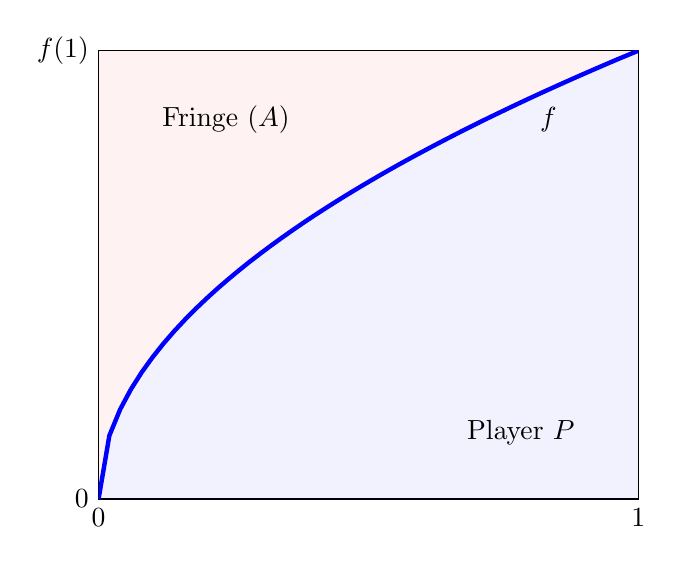
\begin{tikzpicture}
        \begin{axis}[xmin=0, xmax=1, ymin=0, ymax=1, samples at={0, 0.02, ..., 0.98, 1},
                xtick={0, 1}, ytick={0}, extra y ticks={1},  extra y tick style={yticklabel={$f(1)$}}]
            \addplot[name path=f, blue,ultra thick] {x^0.5};
            \node[anchor=north west] at (axis cs: .8, .8^0.5) {$f$};
            \path[name path=bottom] (axis cs:0,0) -- (axis cs:1,0);
            \path[name path=top] (axis cs:0,1) -- (axis cs:1,1);

            \addplot [fill=blue, fill opacity=0.05] fill between [of=f and bottom];
            \addplot [fill=red, fill opacity=0.05] fill between [of=f and top];

            \node[anchor=north west] at (axis cs: .1, .9) {Fringe ($A$)};
            \node[anchor=south east] at (axis cs: .9, .1) {Player $P$};
        \end{axis}
    \end{tikzpicture}
\end{figure}

Finally, the following corollary implies that, even though the individual share of each $A_i$ vanishes as their number goes to infinity, their total value still converges to a positive value.
\begin{corollary}
    \label{cor:fringe_value_2}
    $\varphi_P^\infty < f(1)$ and $\varphi_A^\infty > 0$ for any $f$ that is not constant.
\end{corollary}


\subsection{Weighted Shapley-values}

While the values of oceanic games (i.e. the limits of the Shapley values of their finite approximations in finite games) are well known in the relevant literature, there are no results about the limits of the weighted (Shapley) values. While providing very general results in the form of \textcite[]{fogelman1980asymptotic} is outside of the scope of the paper\footnote{They show that the (within some constraints) any discretization of an oceanic game converges to the same value.} the results in this section still provide some new insights into weighted values of oceanic games. In particular, I show that the weighted value of a game with one large and many small players converges to a rather simple and intuitive expression, if the size of the small players go to zero at the same rate.

Imagine a general non-cooperative game $(N, v)$ with $N = \{1, \dots, n\}$. Assume that, in addition to the value function $v : 2^n \to \mathbb{R}$, the game is also endowed with a weight system $\lambda \in \mathbb{R}^n$. These weights can be thought of as measures of innate bargaining power \parencite{shapley1953additive}, not reflected in the value function. Further support for this interpretation can be found in \textcite{hart1996bargaining}, demonstrating that in a certain alternating offer bargaining game, weights are related to the probability of each player making the offer.\footnote{For example, only one player having a positive value corresponds to them making take it or leave it offers.}

For my purposes, it is sufficient to deal with the case of simple weights. I.e., assume that there is at most one player with zero weight. For my main result, I make use of the fact that weighted Shapley values can be calculated by weighting the permutations by the probabilities arising from the following sequential ordering procedure \parencite{kalai1987weighted}. Start with the set of all players. Let the probability of player $i$ being the last amongst the set of remaining players $R$ be $\lambda_i / \sum_{j \in R} \lambda_j$. Continue until all players are exhausted. This yields a well-defined probability for each permutation of players.

Consider the game described in the previous section, and let the weights of players of type $A$ and $P$ be 1 and $\lambda$, respectively. Let $X_n$ be a random variable representing the number of players before $P$ when players are ordered according to the above procedure. Then, the probability of player $P$ having at most $k$ players of type $A$ before themselves is simply
\begin{align*}
    \Pr{X_n \leq k} = \prod_{j=k+1}^n \frac{j}{j + \lambda} .
\end{align*}
The following lemma establishes the continuous analogue of this statement.
\begin{lemma}
    \label{lem:entry_distr}
     As $n \to \infty$, $X_n \xrightarrow[]{\mathrm{d}} X$ with the cdf $G_X(t) = \lambda^t$. Consequently, the corresponding probability density function is $g(t) = \lambda t^{\lambda - 1}$.
\end{lemma}

The main proposition of this section shows that the weighted Shapley-value of player $i$ can be expressed as the expected marginal contribution of that player where the permutations are weighted according to the previous distribution.
\begin{proposition}
    \label{prop:one_sided_weighted}
    Let $f(t)$ be continuous on $[0, 1]$. Then
    \begin{align*}
        \varphi_P(\lambda, \infty) = \int_0^1 g(t) f(t) \dt
    \end{align*}
    where $g(t) = \lambda t^{\lambda - 1}$.
\end{proposition}

Finally, the following corollaries support the interpretation of weights as bargaining power, as a higher weight corresponds to a higher Shapley-value in this game.\footnote{This would not necessarily have to be the case, as demonstrated by \textcite{owen1968communications}.} Furthermore, the limit of the weighted value of $P$, as their weight goes to zero (infinity) is precisely the payoffs $P$ would achieve if $P$ were making (facing) take-it-or-leave-it offers.

\begin{corollary}
    \label{cor:platform_value_weighted}
    $\varphi_P(\lambda, \infty)$ is increasing in $\lambda$ unless $f$ is constant.
\end{corollary}

\begin{corollary}
    \label{cor:paltform_value_weighted_2}
    If the weight of player $P$ goes to infinity (zero), its weighted Shapley value converges to $f(1)$ ($f(0)$).
\end{corollary}

\subsection{Multiple platforms}

Imagine that, instead of just one, there are $m$ players of type $P$, and they are perfect substitutes of each other. That is, the fringe players still need a platform to achieve any value, but it does not matter which or how many platforms are available for them. Formally, the value function for coalition $S$ is the following:
\begin{align*}
    v(S) = \begin{cases}
        0                              & \text{if } n_P(S) = 0 \\
        f\left(\frac{n_A(S)}{n}\right) & \text{otherwise}.
    \end{cases}
\end{align*}

Let us start by establishing monotonicity for this version of the model, too.
\begin{proposition}
    The game is monotone if $f$ is increasing and $f(0) \geq 0$.
\end{proposition}
% \textcolor{red}{Note: I have to think more about how to describe this situation in the language of cooperative game theory. The issue is that, for example, the value of $\{P_1, A_1\}$ depends on whether $\{P_2, A_2\}$ also decides to form a coalition and enter the market.}

As before, the main proposition in this section provides us with an expression of the limit of the value for this variant of the game.
\begin{proposition}
    \label{prop:multiple_platforms}
    The limit of the Shapley-value (as $n \to \infty$) of each player of type $P$ is
    \begin{align*}
        \varphi_{P_i}^{\infty, m} = \int_0^1 (1-t) ^ {m-1} f(t) \dt .
    \end{align*}
\end{proposition}

As with proposition \ref{prop:one_sided}, this result also has a probabilistic interpretation, and could have been obtained directly using the axiomatic approach. Let the location of the $m$ atoms be $t_1, \dots, t_m$, distributed independently and uniformly on the unit cube. The expected marginal contribution of $t_i$ is only positive whenever it is the first amongst the major players. That is, for any $t_i$, the probability if $P_i$ being the first is related to the cdf of the first order statistic from $n-1$ independent uniform distributions: $1 - (1-t)^{m-1}$.

\begin{corollary}
    \label{cor:multiple_platforms}
    The per-unit Shapley-value of the fringe is
    \begin{align*}
        \varphi_A(k, \infty) = 1 - m\int_0^1 (1-t) ^ {m-1} f(t) \dt = \int_0^1 [1 - (1-t)^m] f'(t) \dt .
    \end{align*}
\end{corollary}

The following corollary again demonstrates that the predicted outcomes confirm intuitions. As the major players become more and more substitutable, the portion of the surplus they can capture decreases, and the aggregated value of the fringe increases.

\begin{corollary}
    \label{cor:multiple_platforms_2}
    Let $\varphi_{P}^{\infty, m} = m\varphi_{P_i}^{\infty, m}$ denote the aggregated values of players of type $P$. $\varphi_{P}^{\infty, m}$ is decreasing in $m$ and $\varphi_{A}^{\infty, m}$ is increasing in $m$ unless $f$ is constant.
\end{corollary}

\section{Two-sided case}

Now imagine that, in addition to player $P$, there are two types of smaller players: $\{A_1, \dots, A_n\}$ and $\{B_1, \dots, B_n\}$. As before, $P$ is necessary for any coalition to have a positive value, and the small players are identical within their groups. I.e., the set of players and the characteristic function of the game are the following: $N = \{P, A_1, \dots, A_n, B_1, \dots, B_n\}$ and
\begin{align*}
    v(S) = \begin{cases}
        0                                                & \text{if } P \notin S \\
        f\left(\frac{n_A(S)}{n}, \frac{n_A(S)}{n}\right) & \text{otherwise}.
    \end{cases}
\end{align*}
A prominent interpretation of this model would be a platform marketplace with a set of sellers and a set of buyers, where all three sides possess some amount of bargaining power. However, player $P$ does not have to be in the ``middle'' of the transactions for this framework to be applicable. For example, it also captures the situation of a single upstream producer, a large number of downstream firms, and a similarly large number of customers, as long as both the customers and the downstream firms can participate in the bargaining process. A setting where these assumptions might be plausible is, for example, the new car market with a car producer, a number of independent dealerships, and customers who might engage in negotiation.

Let us follow the pattern from the previous sections. Start by characterizing conditions for superadditivity to support the bargaining interpretation.
\begin{proposition}
    The game $(N, v)$ is monotone and superadditive if and only if $f$ is increasing in both arguments.
\end{proposition}

Next, let us obtain formulas for the values of the three groups of players. It turns out that the limits of the Shapley-values (as $n \to \infty$) are still analytically tractable and they also have neat interpretations.

\begin{proposition}
    Let $f(a, b)$ be continuous everywhere on $[0, 1]^2$. Then,
    \begin{align*}
        \varphi_P^\infty & = \int_0^1 f(t, t) \dt                                 \\
        \varphi_A^\infty & = \int_0^1 t \frac{\partial f(t, t)}{\partial a} \dt   \\
        \varphi_B^\infty & = \int_0^1 t \frac{\partial f(t, t)}{\partial b} \dt .
    \end{align*}
\end{proposition}

As the previous proposition shows, the value of each kind of player depends on their expected marginal contribution, i.e. the partial derivatives of $f$. Consequently, the value of the grand coalition can be decomposed into the Shapley-values of its members signifying their expected marginal contributions in the following way:
\begin{align*}
    f(1, 1) = \underbrace{\int_0^1 f(t, t) \dt}_{\text{ player } P} + \underbrace{\int_0^1 t \frac{\partial f(t, t)}{\partial a} \dt}_{\text{players } A} + \underbrace{\int_0^1 t \frac{\partial f(t, t)}{\partial b} \dt}_{\text{players } B}.
\end{align*}

One surprising element of the result is that one only has to integrate over the diagonal of the support  of $f$, and the value does not depend on the marginal contributions in the case of an unequal measure of $A$ and $B$ types. The intuition for that relies on a law-of-large-numbers-type reasoning. If the number of fringe players is large, then it is very unlikely that, after a random ordering, their proportion in any interval will be too different. Consequently, when taking the expectation over all orderings, ones with vary unequal numbers of the two types will have little impact on it.


\subsection{Multiple platforms}

The two-sided case can also simply be extended to incorporate multiple platforms instead of just one. As before, assume that there are $k$ players of type $P$ which are perfect substitutes of each other:
\begin{align*}
    v(S) = \begin{cases}
        0                                                & \text{if } P_i \notin S \; \forall \, i = 1, \dots, k \\
        f\left(\frac{n_A(S)}{n}, \frac{n_B(S)}{n}\right) & \text{otherwise}.
    \end{cases}
\end{align*}

It can be shown that the values of each type of player are rather similar to the one-platform case.
\begin{proposition}
    The unit Shapley-values of the various types of players are
    \begin{align*}
        \varphi_{P_i}(k, \infty) & = \int_0^1 (1-t)^{k-1} f(t, t) \dt                                 \\
        \varphi_A(k, \infty)     & = \int_0^1 [1 - (1-t)^k] \frac{\partial f(t, t)}{\partial a} \dt   \\
        \varphi_B(k, \infty)     & = \int_0^1 [1 - (1-t)^k] \frac{\partial f(t, t)}{\partial b} \dt .
    \end{align*}
\end{proposition}

Similarly, as the next corollary demonstrates, the combined value of platforms is still decreasing in their number.
\begin{corollary}
    Let $\varphi_{P}(k, \infty) = k\varphi_{P_i}(k, \infty)$ denote the aggregated Shapley-values of players of type $P$. Then $\varphi_{P}(k, \infty)$ is decreasing in $k$ and $\varphi_{A}(k, \infty)$, $\varphi_{B}(k, \infty)$ is increasing in $k$ unless $f$ is constant.
\end{corollary}


\section{Application}

This section demonstrates the usefulness of the cooperative approach via a model of a hybrid market, based on that in \textcite[]{anderson2021hybrid}. Consider a market with a continuum of firms $a(t)$ ($t \in \mathbb{R}^+$), continuum of identical consumers and one platform $P$. Assume former two can only interact through the platform. Let each firm have its own, differentiated product. The consumers have a logit utility function over these products, and a set of outside options of measure 1. I will examine the outcome in two situations: (1) the platform functions as a pure marketplace without having an own product, and (2) the platform operating in hybrid mode, selling a measure $N_P$ of differentiated products of its own. 

\subsection{Timing of the game}

The game proceeds as follows. In the first stage, each firm decides whether to invest in creating a product or not. Creating a product incurs a development cost of C. Firms that choose not to invest obtain a payoff of 0 and are excluded from the remainder of the game.

Next, the firms that have a product decide whether they want to join the platform at the cost of some entry fee $F^f$. (Note that the entry fee can be negative, in which case it is a subsidy from the platform to the firm.) Consumers are assumed to be on the platform without a choice. Finally, the platform and the entering firms post their product prices, and produce and sell to consumers at marginal cost $c$.

The model heavily depends on how the entry fees are determined. The most widespread assumption in the literature is that they are unilaterally decided by the platform, and are essentially take it or leave it offers for the other players. The issue with this approach is that it generally leads to extreme conclusions (depending on the number of platforms, and assumptions about single-and-multi-homing, the platforms either act as monopolists or obtain zero profits). As an alternative to this, in this paper, I assume that firm entry fees are a result of some bargaining process between the firms and the platform. Furthermore, the bargaining process is such that it leads to an allocation in which the final profits of each player correspond to their Shapley values.

The characteristic function (necessary for computing values) of a coalition consisting of the platform and any set of firms is defined as follows. Take the members of any given coalition as fixed. Let firms and the platform set profit-maximizing prices for their products without collusion. Note that these prices will be irrespective irrespective of earlier decisions, as both development costs and entry fees are sunk cost at this point. The total profits of the coalition is then the sum of the platform's and the firms' profits from product sales.

While the previous procedure might look somewhat peculiar at first glance, its elements would not be out of place in more traditional (non-cooperative) models, either. Principally, the two main ideas it relies are the following. First, bargaining outcomes should not depend on which player actually obtains the money, all that matters is the total that a given set of players can obtain.\footnote{For example, imagine the following two situations with two players. In the first one, the first player obtains a playoff of two dollars if they both decide to cooperate and nothing otherwise. In the second scenario, both players receive one dollar in the case of cooperation. If they can transfer monay between each other, bargaining outcomes should be the same in both scenarios.} Second, players during the bargaining foresee the (unique) subgame perfect equilibrium in the following subgame, and negotiate based on them.

\subsection{The pricing subgame}

Let us start from the last stage, when firms' entry to the platform is already decided: a measure $N_f$ of firms is present on the platform. Assume that consumers have the same Logit-form demand system as in \textcite{anderson2021hybrid}. Each consumer buys precisely a measure one of products, those giving her the highest net utility. The utility from choosing outside option $i$ is $\mu \epsilon_{0i}$. The net utility from buying the platform's $i$th product at price $p_{Pi}$ is $v - p_{Pi} + \mu \epsilon_{Pi}$, while the net utility from choosing the $i$th fringe firm's product is $v - p_{Fi} + \epsilon_{Fi}$. $\epsilon_{Pi}, \epsilon_{Fi}$ and $\epsilon_{0i}$ come from identical, independent, standardized Gumbel-distributions.

As shown in \textcite{anderson2021hybrid}, the demand for each of these three types of products is
\begin{align*}
    q_{Pi} &= \frac{\int_0^{N_P}  e^\frac{v - p_{Pi} \di}{\mu}}{A} \\
    q_{Fi} &= \frac{e^\frac{v - p_{Fi}}{\mu}}{A} \\
    q_{0i} &= \frac{1}{A} .
\end{align*}
where
\begin{align*}
    A = \int_0^{N_P} e^\frac{v - p_{Pi}}{\mu} \dt + \int_0^{N_F} e^\frac{v - p_{Fi}}{\mu} \dt + 1.
\end{align*}

Furthermore, it can be shown that the optimal pricing strategy is a constant, additive markup over the unit cost. Moreover, the markup is the same for both the platform and the firms, and corresponds to the dispersion in tastes:
\begin{align*}
    p_{Pi} = p_{Fi} = c + \mu.
\end{align*}

Conversely, the profit of the two types of players are
\begin{align*}
    \pi_{Fi} &= \frac{\mu}{A} e^\frac{v - c - \mu}{\mu} \\
    \pi_{Pi} &= N_P \frac{\mu}{A} e^\frac{v - c - \mu}{\mu}
\end{align*}
and the total profits of all players together are
\begin{align*}
    v(N_f) = N_f \pi_{Fi} + \pi_{Pi} = \mu \frac{A - 1}{A}.
\end{align*}

Let $B = e^\frac{v - c - \mu}{\mu}$. Then the total profits from sales (platform and firms combined) can be expressed as
\begin{align*}
    v(N_f) = \frac{N_P B + N_f B}{N_P B + N_f B + 1}.
\end{align*}
This is the characteristic function that forms the basis of the profit allocation. 

\subsection{Deciding firm entry fees}

Let us look at the second stage of the game: firms have made their investment decisions, and are now negotiating with the platform over the entry price. Let us assume that $\bar{N}_f \in \mathbb{R}^+$ measure of firms have made an investment. $C$ is a fixed cost, therefore does not influence the rest of the game. It is simpler to think about bargaining final net profits (entry fees can always be set to achieve any final allocation of profits), which are assumed to be equal to the players' Shapley values. Let us denote these values by $\varphi_f(v, T)$ and $\varphi_P(v, T)$ for the firms and the platform, respectively. As shown in proposition \ref{prop:one_sided},
\begin{align*}
    \varphi_P(v, \bar{N}_f) &= \int_0^1 v(t \bar{N}_f) \dt \\
    &= 1 - \frac{\log(BN_p + BN_f + 1) - \log(BN_p + 1)}{BN_f}
\end{align*}
and
\begin{align*}
    \varphi_f(v, \bar{N}_f) &= v(\bar{N}_f) - \int_0^1 v(t \bar{N}_f) \dt \\
    &= \frac{N_P B + N_f B}{N_P B + N_f B + 1} - 1 + \frac{\log(BN_P + BN_f + 1) - \log(BN_P + 1)}{BN_f} \\
    &= \frac{\log(BN_P + BN_f + 1) - \log(BN_P + 1)}{BN_f} - \frac{1}{N_P B + N_f B + 1}.
\end{align*}

\subsection{Equilibrium entry}

Finally, looking at the first stage, firms will make the initial investment if and only if $\varphi_{f_i}(v, \bar{N}_f) = \varphi_f(v, \bar{N}_f) / \bar{N}_f \geq C$. Therefore, because of the free entry condition, the equilibrium measure of entrants is given by the equation
\begin{align*}
    \underbrace{\frac{\log(BN_P + B\bar N_f + 1) - \log(BN_P + 1)}{B\bar N_f} - \frac{1}{N_P B + \bar N_f B + 1}}_{\equiv h(\bar N_f)} = C \bar{N}_f.
\end{align*}

Let us examine the implications of this result through a numerical example. Let $B=1, C=0.2$, and let the product variety of the platform be $0$ and $0.2$ in the pure marketplace and the hybrid case, respectively. The equilibrium number of entrants is shown in figure \ref{fig:entry}.
\begin{figure}
    \centering
    \includegraphics[width=4in]{out/figures/equilibrium_nf.png}
    \caption{Equilibrium number of fringe entrants as a function of the platform's product variety.}
    \label{fig:entry}
\end{figure}

It is immediately apparent from the figure, that a platform operating in hybrid mode discourages fringe entry, as a direct result of more competition and lower profits in the final stage of the game. However, a more subtle point is that the total number of products (platform's products plus measure of entrants) is also lower in the hybrid case. Because consumer surplus is proportional to the logarithm of the number of available products, this also corresponds to a decrease in that measure.

 In the version of the model without bargaining, the platforms' product variety does not influence total product variety, as long as entry fees are fixed. An increase in the monopolist's product variety will lead to an identically sized decrease in fringe entry, leaving the total number of available products, and, conversely, consumer welfare, unchanged. Operating in hybrid mode only influences fringe entry through more indirect channels, e.g. self-preferencing \parencite[]{hagiu2022should} or distorted incentives when setting revenue-based fees \parencite[]{anderson2021hybrid}. This example application highlights another channel of distortion created by hybrid platforms: a platform having its own products has more bargaining power when entry fees are determined, leading to lower fringe profits. As a consequence, fewer firms enter than in the pure marketplace scenario, and this decrease is more significant than the addition of the platform's own products.

\section{Conclusions}

This paper proposed a new framework to think about the profit allocation in situations concerning a few large and a continuum of smaller players. The results are especially relevant for upstream-downstream situations, platform settings, and two-sided markets. The outcomes of the Shapley-value-based gain sharing rule generally concur with intuitive expectations, and the resulting formulas are more tractable than most explicit non-cooperative approaches.

The illustrative hybrid platform model also highlights the strengths of this approach. Despite its simplicity, it highlights a novel channel through which platforms selling their own products might lead to welfare losses: hybrid platforms have more bargaining power against potential entrants than traditional ones. This mechanism should probably also be considered when competition authorities assess mergers between platforms and contents providers.

There is a variety of ways through which this paper could be expanded or built upon. On the theoretical side, some of the stricter assumptions could be relaxed, such as fringe agents achieving a zero payoff without the platform. Besides, the convergence result for the weighted values could be strengthened if one could manage to show that any sequence along ever more refined partitions of the atomic players converges to the same limit \parencite[à la][]{fogelman1980asymptotic}. The possibilities for practical applications are no less interesting, either. As a first step, the majorly simplified example application could be expanded upon, so that it is a better description of certain real-life paltform markets. Finally, the cooperative approach to profit distribution could become an alternative for the more usual, but in some sense more extreme assumptions about the bargaining process widely used in industrial organization models.

% Next steps:
% \begin{itemize}
%     \item Show how the equilibrium number of entrants depends on $N_P$
%     \item Show how consumer welfare (which is proportional to $\log(N_f + N_P)$) depends on $N_P$
%     \item Try to characterize the profit-maximizing $N_P$ and how it depends on the parameters
% \end{itemize}

\appendix

\printbibliography

\section{Miscellaneous lemmas}

\begin{lemma}
    \label{lemma:log_convergence}
    Let 
    \begin{align*}
        \Delta_n(s) &= \frac{\log(s + 1/n) - \log(\lambda)}{n}, \\
        \Delta(s) &= \frac{1}{s}.
    \end{align*}
    Then $\Delta_n \xrightarrow[]{\mathrm{u}} \Delta$ uniformly on $[t, 1]$ for any $t > 0, \lambda > 0$.
\end{lemma}
\begin{proof}[Proof of Lemma \ref{lemma:log_convergence}]
    First, note that $\Delta_n$ and $\Delta$ are all continuous functions. Then, following the standard proof for $\frac{\mathrm{d}}{\mathrm{d}s}log(s) = \frac{1}{s}$ rewrite $\Delta_n(s)$ as
    \begin{align*}
        \Delta_n(s) &= \frac{\log(s + 1/n) - \log(\lambda)}{n} \\
        &= \log \left( 1 + \frac{1}{sn} \right) ^ n .
    \end{align*}
    It is well known that $\left( 1 + \frac{1}{sn} \right) ^ n$ is monotone increasing in $n$ and converges to $\exp (1/s)$. Therefore, the pointwise convergence of $\Delta_n(s) \to \Delta(s)$ is also monotone.

    Finally, by Dini's theorem, the monotone pointwise convergence of a sequence of continuous functions to a continuous function on a compact set implies uniform convergence on that set.
\end{proof}

\begin{lemma}
    \label{lemma:integral_convergence}
    Let $f_n, f: [a, b] -> \mathbb{R}$ be Riemann-integrable functions with $f_n \xrightarrow[]{\mathrm{u}} f$ uniformly. Then,
    \begin{align*}
        \lim_{n \to \infty} \frac{b-a}{n} \sum_{k=1}^n f_n \left( a + \frac{b-a}{n} \right) = \int_0^1 f(t) \dt.
    \end{align*}
\end{lemma}
\begin{proof}[Proof of Lemma \ref{lemma:integral_convergence}]
    \begin{align*}
        &\lim_{n \to \infty} \frac{b-a}{n} \sum_{k=1}^n f_n \left( a + \frac{b-a}{n} \right) \\
        &= \lim_{n \to \infty} \frac{b-a}{n} \left[ \sum_{k=1}^n f \left( a + \frac{b-a}{n} \right) + \sum_{k=1}^n \left( f_n \left( a + \frac{b-a}{n} \right) - f \left( a + \frac{b-a}{n} \right) \right) \right] \\
        &= \int_a^b f(t) \dt + \lim_{n \to \infty} \frac{b-a}{n}\sum_{k=1}^n \left( f_n \left( a + \frac{b-a}{n} \right) - f \left( a + \frac{b-a}{n} \right) \right) \\
        &\leq \int_a^b f(t) \dt + \lim_{n \to \infty} \frac{b-a}{n}\sum_{k=1}^n \left| f_n \left( a + \frac{b-a}{n} \right) - f \left( a + \frac{b-a}{n} \right) \right| \\
        &\leq \int_a^b f(t) \dt + \lim_{n \to \infty} \frac{b-a}{n}\sum_{k=1}^n \sup_{t \in [a, b]} \left| f_n(t) - f(t) \right| \\
        &= \int_a^b f(t) \dt + (b-a) \underbrace{\lim_{n \to \infty} \sup_{t \in [a, b]} \left| f_n(t) - f(t) \right|}_{=0 \text{ due to uniform convergence}} \\
        &= \int_a^b f(t) \dt
    \end{align*}
\end{proof}


\section{Proofs of propositions and lemmas in the main text}

\begin{proof}[Proof of Proposition \ref{prop:monotone}]
    Monotonicity is evident. For superadditivity, note that for any coalitions $S_1, s_2$ such that $S_1 \cap s_2 = \emptyset$, $P \notin S_1$ or $P \notin s_2$. WLOG assume it is the latter, therefore $v(S_2) = 0$. As a result, $v(S_1) + v(S_2) = v(S_1) \leq v(S_1 \cup S_2)$ holds if and only if $(N, v)$ is monotone.
\end{proof}

\begin{proof}[Proof of Proposition \ref{prop:one_sided}]
    Let $R$ denote a permutation of the set of players ($N$). Additionally, let us denote the players preceding $i$ by $\mathcal{P}_i^R$. The value of player $P$ is their expected marginal contribution averaged over all permutations of $N$:
    \begin{align*}
        \varphi_P^n = \frac{1}{(n+1)!} \sum_R v(\mathcal{P}_P^R \cup \{i\}) - v(\mathcal{P}_P^R)
    \end{align*}
    First, note that $v(\mathcal{P}_P^R) = 0$ for any permutation, as no coalition can achieve a positive value without player $P$. Furthermore, using the fact that all agents of type $A$ are identical implies that $v(\mathcal{P}_P^R \cup \{i\})$ only depends on the number of agents in the coalition. More precisely, 
    \begin{align*}
        v(\mathcal{P}_P^R \cup \{i\}) = f(n_A(\mathcal{P}_P^R \cup \{i\}) / n) = f(|\mathcal{P}_P^R| / n).
    \end{align*}
    Finally, the set of permutations in which $k$ number of players precede $P$ is independent of $n$, i.e.
    \begin{align*}
        \{R \mid |\mathcal{P}_P^R| = k\} = n! \quad \forall\, k.
    \end{align*}
    Putting all the above together, the value of player $P$ can be expressed as
    \begin{align*}
        \varphi_P^n &= \frac{1}{(n+1)!} \sum_{k=0}^n n! f(k / n) \\
        &= \frac{1}{n+1} \sum_{k=0}^n f(k / n) \\
        &= \frac{n}{n+1} \underbrace{\frac{1}{n} \sum_{k=0}^{n-1} f(k / n)}_{=S_n} + \frac{1}{n+1} f(1).
    \end{align*}
    $S_n$ are just the left Riemann-sums of function $f$ on the interval $[0, 1]$. Therefore, if $f$ is continuous (and thus Riemann-integrable), then $S_n \to \int_0^1 f(t)$, and thus
    \begin{align*}
        \lim_{n \to \infty} \varphi_P^n &= \lim_{n \to \infty} \frac{1}{n+1} \sum_{k=1}^n f(k / n) \\
        &= \lim_{n \to \infty}\underbrace{\frac{n}{n+1}}_{\to 1} \frac{1}{n} \sum_{k=0}^{n-1} f(k / n) + \underbrace{\frac{1}{n+1} f(1)}_{\to 0} \\
        &= \int_0^1 f(t) \dt .
    \end{align*}
\end{proof}

\begin{proof}[Proof of Corollary \ref{cor:fringe_value}]
    The first equality comes from the efficiency of the Shapley-value. The values of all players sum up to $f(1)$ for all $n \in \mathbb{N}$, therefore
    \begin{align*}
        \lim_{n \to \infty} \sum_{i=1}^n \varphi_{A_i}^n = \lim_{n \to \infty} (1 - \varphi_P^n ) = 1 - \int_0^1 f(t).
    \end{align*}
    The second can be obtained by integration by parts:
    \begin{align*}
        \int_0^1 t f'(t) \dt = tf(t) \mid_0^1 - \int_0^1 f(t) \dt = f(1) - \int_0^1 f(t) \dt
    \end{align*}
\end{proof}

\begin{proof}[Proof of Lemma \ref{lem:entry_distr}] %\textcolor{red}{(Might have to fix sum indices)} \\
    The probability of $P$ having at most fraction $t$ of the other players before itself is
    \begin{align*}
        \Pr(X_n \leq nt) &= \Pr(X_n \leq nt ) \\
        &= \prod_{j = nt + 1}^n \frac{j}{j + \lambda} \\
        &= \exp \Bigg( \underbrace{\sum_{j = nt + 1}^n \log(j) - \log(j+\lambda)}_{\equiv S_n} \Bigg).
    \end{align*}
    Taking limits,
    \begin{align*}
        \lim_{n \to \infty} S_n &= \lim_{n \to \infty} \sum_{j = nt + 1}^n \log(j) - \log(j+\lambda) \\
        &= \lim_{n \to \infty} \sum_{i = 1}^{n - nt} \log(nt + i) - \log(nt + i + \lambda) \\
        &= \lim_{n \to \infty} \frac{1}{n - nt} \sum_{i = 1}^{n - nt} \frac{\log \left( t + \frac{i}{n - nt} \right) - \log \left( t + \frac{i}{n - nt} + \frac{\lambda}{n - nt} \right)}{1 / (n - nt)}
    \end{align*}
    Let
    \begin{align*}
        \Delta_n(s) = \frac{\log \left( s \right) - \log \left( s + \frac{\lambda}{n - nt} \right)}{1 / (n - nt)}
    \end{align*}
    By lemma \ref{lemma:log_convergence}, 
    \begin{align*}
        \Delta_n \xrightarrow[]{\mathrm{u}} \lambda \frac{\mathrm{d}}{\mathrm{d}s}log(s) = -\frac{\lambda}{s}
    \end{align*}
    on the compact interval $[t, 1]$ for any $t > 0$ ($\xrightarrow[]{\mathrm{u}}$ denotes uniform convergence).
    
    Then, by lemma \ref{lemma:integral_convergence}, we have that
    \begin{align*}
        \lim_{n \to \infty} S_n &= \lim_{n \to \infty} \frac{1}{n-nt} \sum_{i=1}^{n-nt} \Delta_n \left( t + \frac{i}{n - nt} \right) \\
        &= \int_t^1 (\lim_{n \to \infty} \Delta_n)(s) \ds \\
        &= \int_t^1 \lim_{n \to \infty} -\frac{\lambda}{s} \ds \\
        &= \lambda \log{t}
    \end{align*}

    Substituting $\lim_{n \to \infty} S_n$ into the original equation yields
    \begin{align*}
        \lim \Pr \left( \frac{X_n}{n} \leq t \right) &= \exp \Bigg( \lim_{n \to \infty} \sum_{j = nt + 1}^n \log(j) - \log(j+\lambda) \Bigg) \\
        &= \exp(\lambda \log(t)) \\
        &= t^\lambda.
    \end{align*}

    For $t=0$, simply observe that %\textcolor{red}{Have to elaborate on this}
    \begin{align*}
        \lim_{n \to \infty} \prod_{j = 1}^n \frac{j}{j + \lambda} = 0 = 0^\lambda.
    \end{align*}
\end{proof}

\begin{proof}[Proof of Corollary \ref{cor:fringe_value_2}]
    If $f$ is monotone increasing, then $f(0) \leq \int_0^1 f(t) \dt \leq f(1)$. The inequalities become strict if $f$ is not constant on the whole interval.
\end{proof}

\begin{proof}[Proof of Proposition \ref{prop:one_sided_weighted}]
    The weighted value of player $P$ is its expected contribution across all permutations, with each permutation weighted by its probability of occurring.
    \begin{align*}
        \varphi_P^{n, \lambda} = \sum_R \Pr(R) [v(\mathcal{P}_P^R \cup \{i\}) - v(\mathcal{P}_P^R)]
    \end{align*}
    As before, using the fact that fringe players are identical, this can be rephrased as
    \begin{align*}
        \varphi_P^{n, \lambda} &= \sum_{k=0}^n \Pr(R) f(k/n) \\
        &= \E[f(X_n / n)]
    \end{align*}
    where $X_n$ is defined as above. $f$ is continuous, and therefore bounded on the compact set $[0, 1]$. As a consequence, $\frac{X_n}{n} \xrightarrow[]{\mathrm{d}} X$ implies $\E[f(X_n / n)] \to \E[f(X)]$, which in turn gives
    \begin{align*}
        \lim_{n \to \infty} \varphi_P^{n, \lambda} &= \lim_{n \to \infty} \E[f(X_n / n)] \\
        &= \E[f(X)] \\
        &= \int_0^1 f(t) \mathrm{d}G(t) \\
        &= \int_0^1 g(t)f(t) \dt
    \end{align*}
    where $G(t)$ and $g(t)$ are the cdf and pdf of X, respectively.
\end{proof}

\begin{proof}[Proof of Corollary \ref{cor:platform_value_weighted}]
    Let $X$ and $X'$ be random variables with cdfs $G_X = t^\lambda$ and $G_{X'}t^{\lambda'}$, respectively. For any $\lambda < \lambda'$, $t^\lambda > t^{\lambda'} \forall t \in [0, 1]$, meaning that $X'$ first-order stochastically dominates $X'$. As a result, for any monotonically increasing $f$,
    \begin{align*}
        \int_0^1 g_X(t)f(t) \dt = \E[f(X)] \leq \E[f(X')] = \int_0^1 g_{X'}(t)f(t)
    \end{align*}
    with strict inequality unless $f$ is constant almost everywhere. As $f$ is continuous, the latter is equivalent to $f$ being constant on the whole $[0, 1]$ interval.
\end{proof}

\begin{proof}[Proof of Corollary \ref{cor:paltform_value_weighted_2}]
    As $\lambda \to 0$, $X$ converges to the degenerate random variable $X_0$ for which $\Pr(X_0 = 0) = 1$. As a consequence, the expected value of $f(X)$ converges to $\E[f(X_0)] = f(0)$. $\lim_{\lambda \to \infty} \varphi^{\infty, \lambda}_P = f(1)$ can be shown along the same lines.
\end{proof}

\begin{proof}[Proof of Proposition \ref{prop:multiple_platforms}]
    \label{prop:one_sided_multiple}
    First, let us rewrite the expected marginal contribution of player $P_i$ in the following way:
    \begin{align*}
        \varphi_{P_i}^{n, m} &= \frac{1}{(n+m)!} \sum_R v(\mathcal{P}_{P_i}^R \cup \{i\}) - v(\mathcal{P}_{P_i}^R) \\
        &= \frac{1}{(n+m)!} \left[ \sum_{\{R | n_P(\mathcal{P}_{P_i}^R = 0)\}} \left[v(\mathcal{P}_{P_i}^R \cup \{i\}) - v(\mathcal{P}_{P_i}^R)\right] + \sum_{\{R | n_P(\mathcal{P}_{P_i}^R > 0)\}} \left[v(\mathcal{P}_{P_i}^R \cup \{i\}) - v(\mathcal{P}_{P_i}^R)\right] \right]
    \end{align*}
    Next, make use of the fact that the marginal contribution of a platform is zero if another platform is already present, and only depends on the number of fringe firms otherwise.
    \begin{align*}
        \varphi_{P_i}^{n, m} &= \frac{1}{(n+m)!} \sum_{\{R | n_P(\mathcal{P}_{P_i}^R = 0)\}} f (\mathcal{P}_{A}^R / n) \\
        &= \frac{1}{(n+m)!} \sum_{k=0}^n |\{R | n_A(\mathcal{P}^R_{P_i} = k) \text{ and } n_P(\mathcal{P}^R_{P_i} = 0)\}| f(k/n)
    \end{align*}
    Finally, notice that, while the permutations with $k$ fringe agents before $P_i$ does not depend on $k$, amongst those, the number of permutations with no platform before $P_i$ does depend on it. In particular,
    \begin{align*}
        |\{R | n_A(\mathcal{P}^R_{P_i} = k) \text{ and } n_P(\mathcal{P}^R_{P_i} = 0)\}| &= \frac{n!(n+m-k-1)!}{(n-k)!}
    \end{align*}
    and
    \begin{align*}
        \varphi_{P_i}^{n, m} &= \sum_{k=0}^n \frac{n!(n+m-k-1)!}{(n+m)!(n-k)!} f(k/n) \\
        &= \sum_{k=0}^n \frac{(n-k+1)(n-k+2) \dots (n-k+m-1)}{(n+1)(n+2) \dots (n+m)} f(k/n) \\
        &= \frac{1}{n+1}\sum_{k=0}^n \underbrace{\frac{(n(1-k/n)+1)(n(1-k/n)+2) \dots (n(1-k/n)+m-1)}{(n+2) \dots (n+m)} f(k/n)}_{S_n}
    \end{align*}
    For any $t = k/n \in [0, 1]$, 
    \begin{align*}
        S_n(t) \to (1-t)^{m-1}f(t) \equiv S(t).
    \end{align*}
    Furthermore, it is simple to verify that this convergence is uniform, and that $S_n$ and $S$ are all continuous functions. By Dini's theorem, the former properties imply that $S_n \xrightarrow[]{\mathrm{u}} S$ uniformly on $[0, 1]$.

    The conclusion of the proof is similar to that of proposition \ref{prop:one_sided}:
    \begin{align*}
        \lim_{n \to \infty} \varphi_{P_i}^{n, m} &= \lim_{n \to \infty} \underbrace{\frac{n}{n+1}}_{\to 1} \sum_{k=0}^{n-1} S_k(k/n) + \underbrace{\frac{1}{1+n}S(1)}_{\to 0} \\
        &= \lim_{n \to \infty} \sum_{k=0}^{n-1} S_k(k/n) \\
        &= \int_0^1 (1-t)^{m-1} f(t) \dt
    \end{align*}
    with the last equality supported by lemma \ref{lemma:integral_convergence}.
\end{proof}

\begin{proof}[Proof of Corollary \ref{cor:multiple_platforms}]
    The allocation is efficient for all $n \in \mathbb{N}$, therefore efficient in the limit, as well. The second equality can be obtained by integration by parts.
\end{proof}

\begin{proof}[Proof of Corollary \ref{cor:multiple_platforms_2}] (Assuming $f$ is continuously differentiable) %\textcolor{red}{(Assuming $f$ is continuously differentiable -- will have to relax this)}
    $f'(t)$ is non-negative, so $[1 - (1-t)^m] f'(t)$ is increasing in $m$ $\forall t \in [0, 1]$. As a consequence, $\varphi_A^{n, \infty}$ is also increasing in $m$ if $f'(t)$ is positive on some interval or, $f(t)$ is not constant. Conversely, $\varphi_{P}^{\infty, m} = 1 - \varphi_{A}^{\infty, m}$ is decreasing in $m$.
\end{proof}

\end{document}